\section{Análisis}

El primer experimento que creímos útil es la prueba de suficientes combinaciones significativas de valores de $\alpha$ y $\beta$ para intentar identificar un par de valores de óptimo comportamiento. Esto lo hicimos fijando otras variables en algunos valores que nos parecieron coherentes (delay de 2 segundos y sin indeterminismo en los dropeos), para sólamente mirar dichas variables.\\

\indent Para poder evaluar esto, elegimos valores entre 0.1 y 0.9, aumentando en cada paso en 0.1 la variable analizada. Probamos algunos valores en el medio pero consideramos que aumentar la granularidad no nos daría cambios significativos en los resultados. Esto nos da una matríz de 81 resultados, los cuales, para poder analizarlos, partimos en 9 gráficos\footnote{Aparte de estas imágenes, debajo de cada uno se encuentra un link a su versión interactiva, para poder apreciar mejor los datos.}, fijando cada valor de $\alpha$ y graficando las variaciones de los $\beta$.\\

\indent En todos los gráficos, aparte del resultado de cada $\beta$ con el $\alpha$ de dicha corrida, se encuentra una línea constante que representa el \textbf{promedio de RTT} el cual en el caso ideal, sería el mismo valor que el \textbf{RTO}. La elección de mejor par de $\alpha$ y $\beta$ la hicimos bajo este criterio, viendo para cada valor de $\alpha$, el valor de $\beta$ que más rápido llega a parecerse al RTT promedio y el que más estable se mantiene a lo largo de las pruebas (pues puede que alguno llegue rápido pero luego de algunas iteraciones empiece a mostrar comportamiento errático y no sea tan bueno en general).

\begin{center}
	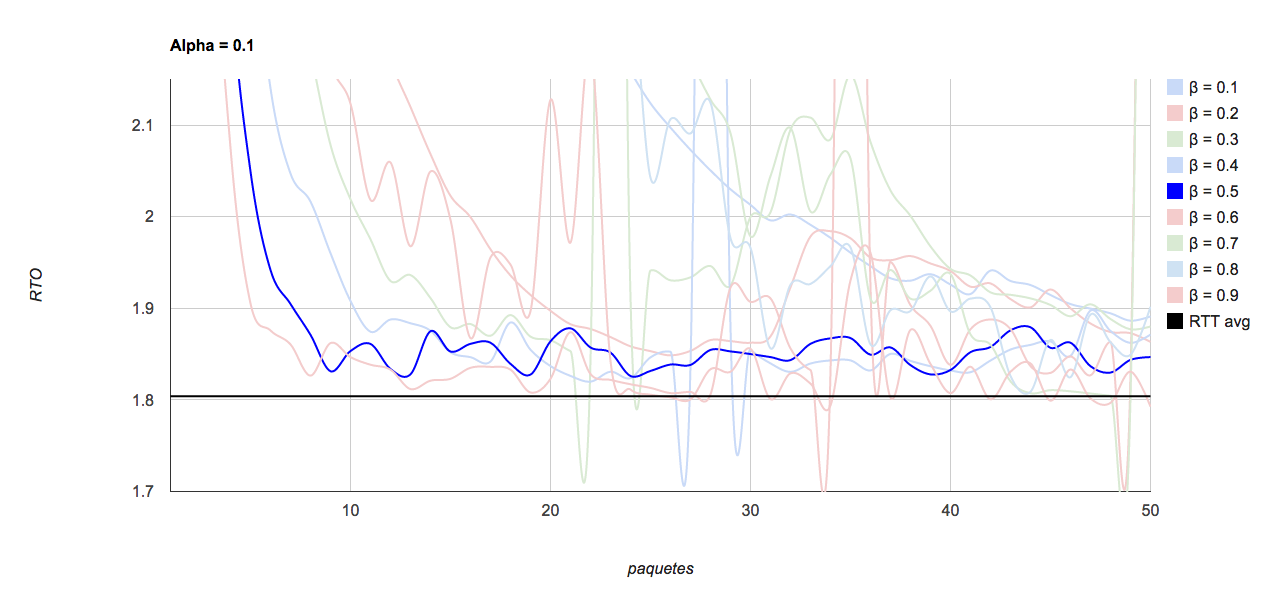
\includegraphics[scale=0.35]{graphics/rto_vs_paquetes_a_1.png}
	\textit{Gráfico interactivo en:} http://goo.gl/i3q8vd
\end{center}

\begin{center}
	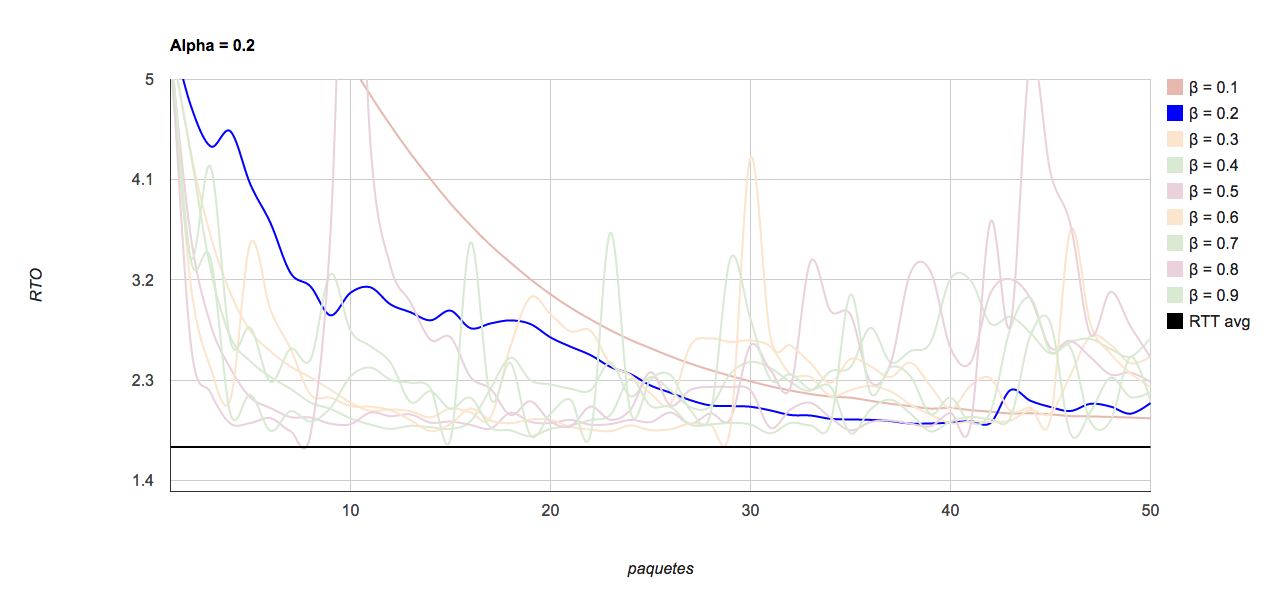
\includegraphics[scale=0.35]{graphics/rto_vs_paquetes_a_2.png}
	\textit{Gráfico interactivo en:} http://goo.gl/QS0NjO
\end{center}

\begin{center}
	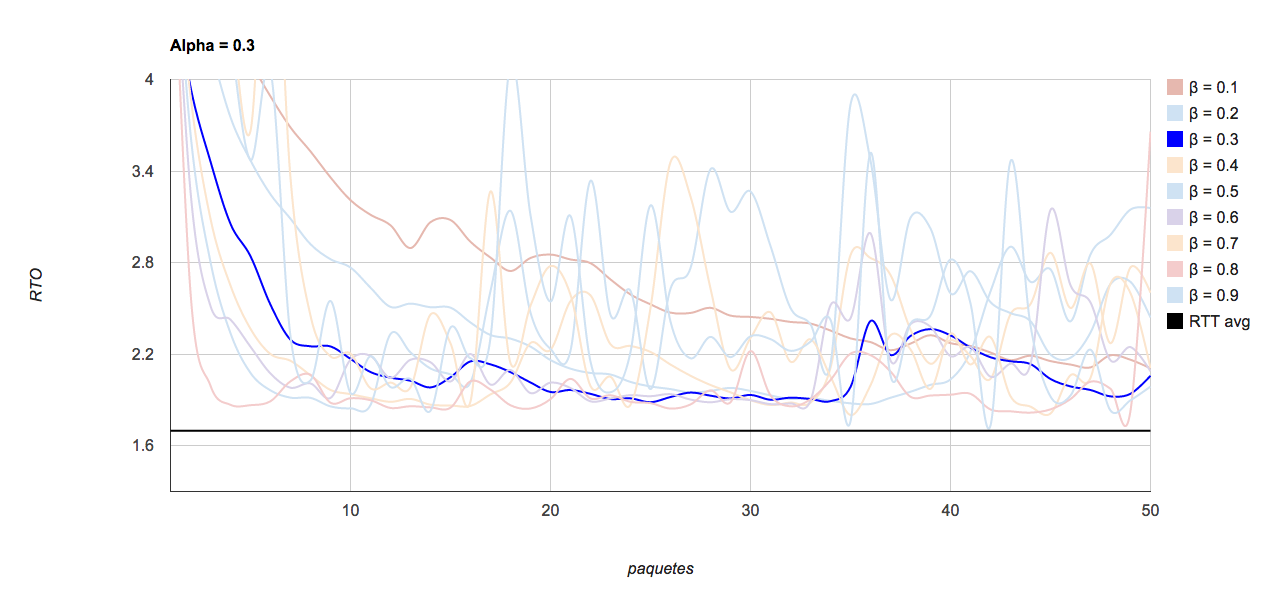
\includegraphics[scale=0.35]{graphics/rto_vs_paquetes_a_3.png}
	\textit{Gráfico interactivo en:} http://goo.gl/cmSyGd
\end{center}

\begin{center}
	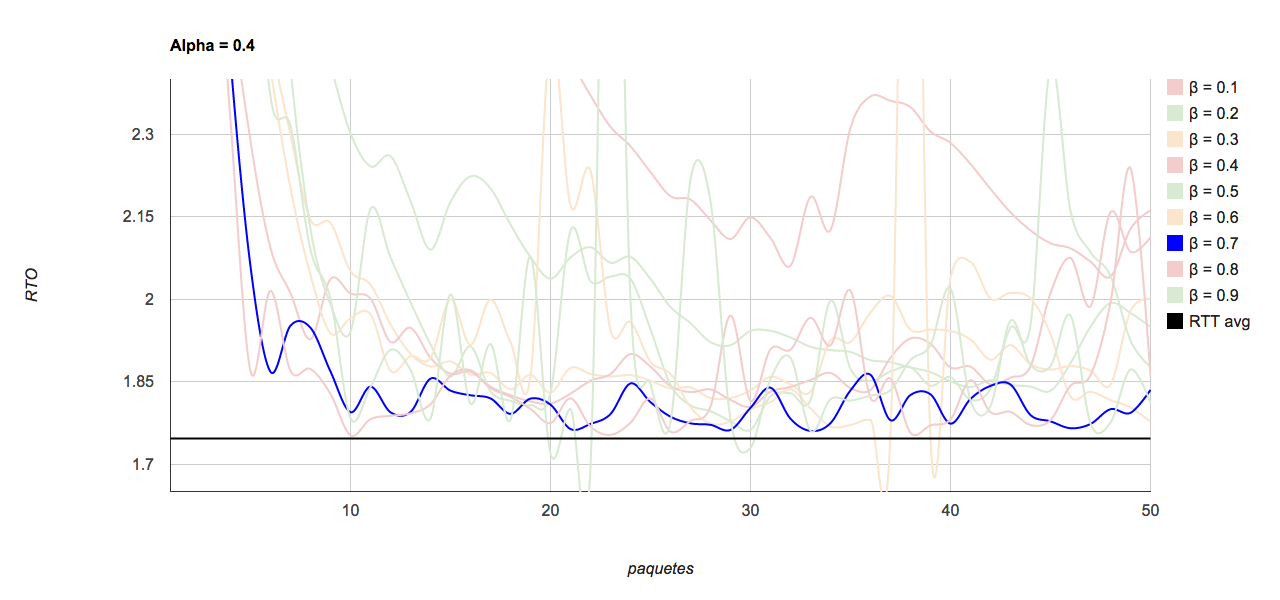
\includegraphics[scale=0.35]{graphics/rto_vs_paquetes_a_4.png}
	\textit{Gráfico interactivo en:} http://goo.gl/Db08yU
\end{center}

\begin{center}
	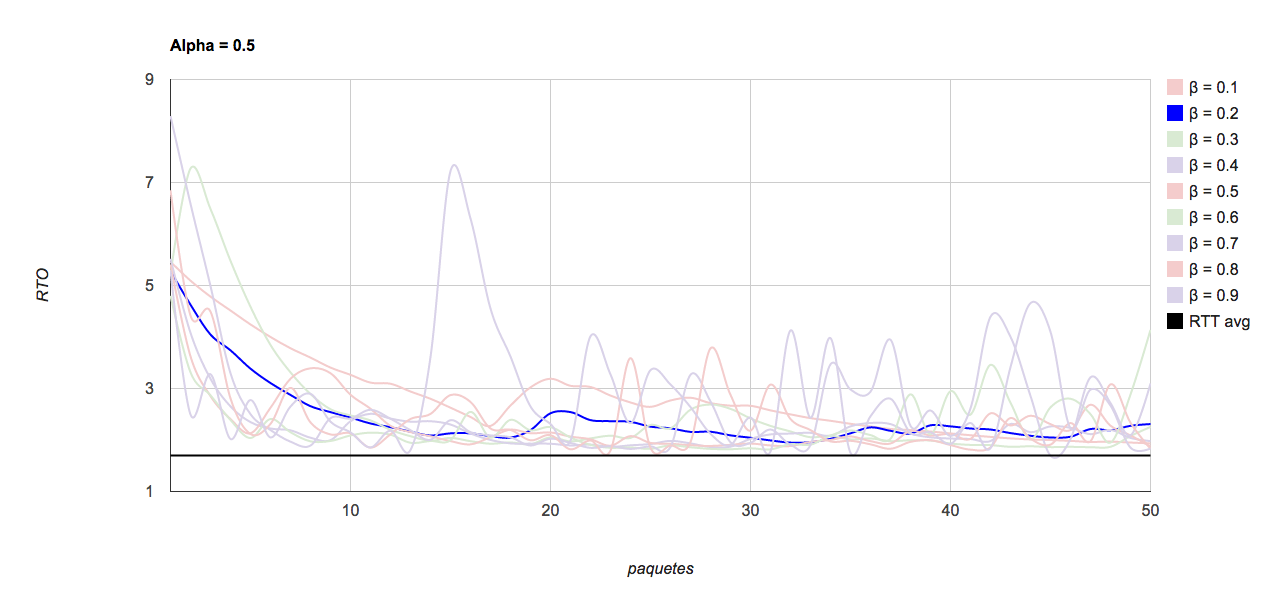
\includegraphics[scale=0.35]{graphics/rto_vs_paquetes_a_5.png}
	\textit{Gráfico interactivo en:} http://goo.gl/VNV8xF
\end{center}

\begin{center}
	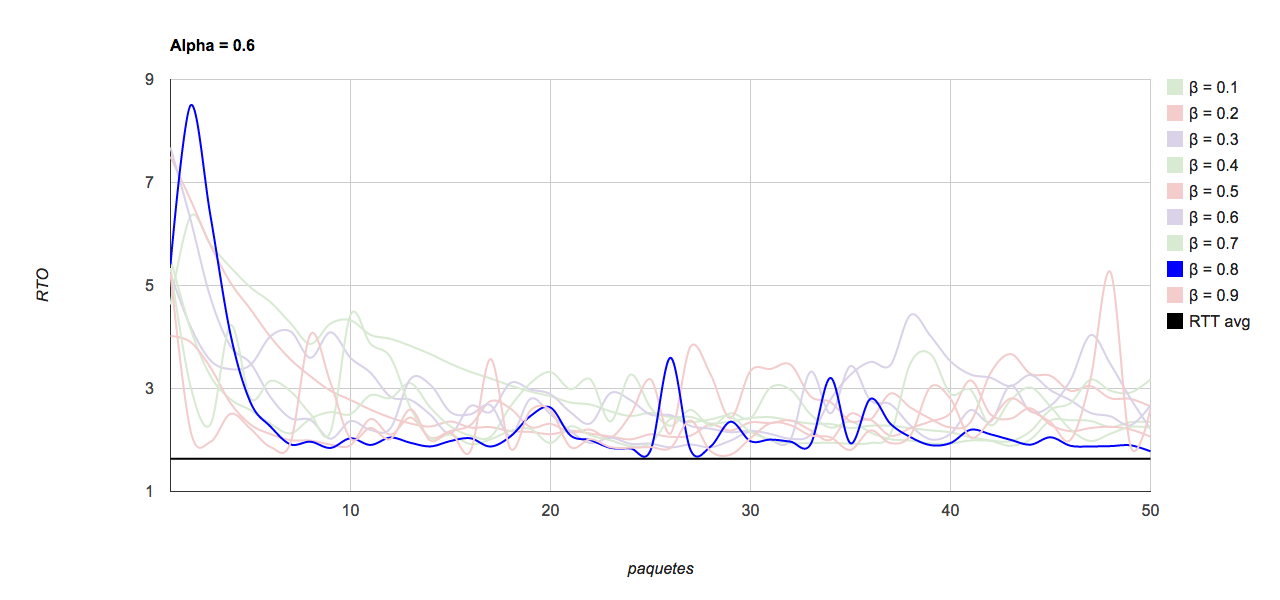
\includegraphics[scale=0.35]{graphics/rto_vs_paquetes_a_6.png}
	\textit{Gráfico interactivo en:} http://goo.gl/CN4joc
\end{center}

\begin{center}
	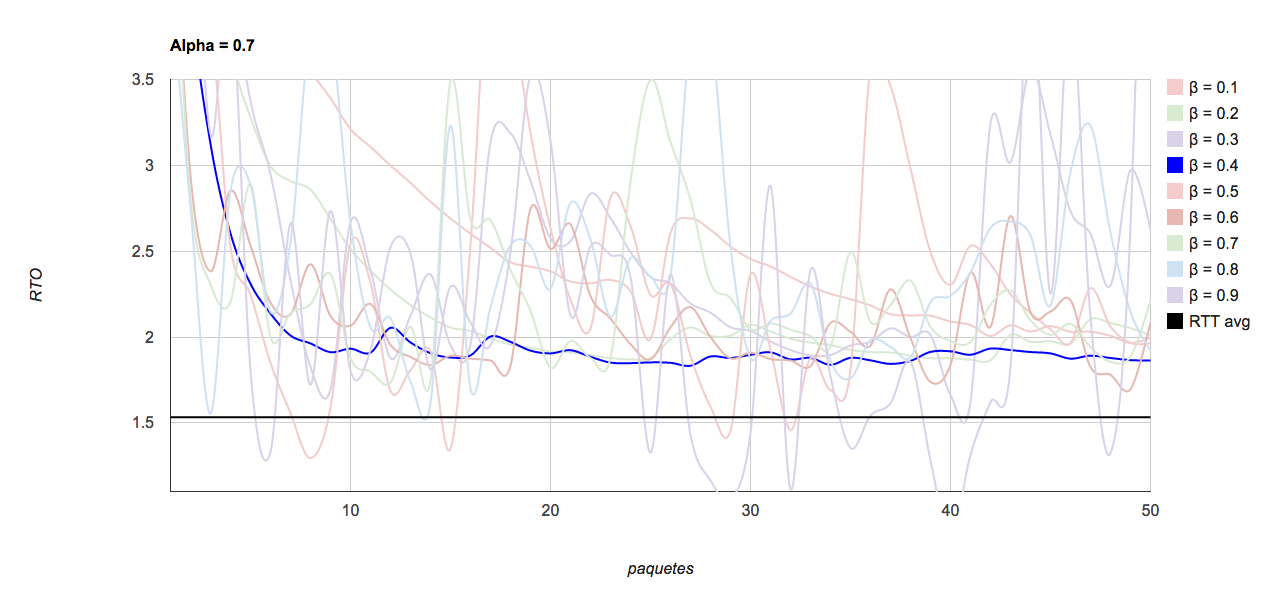
\includegraphics[scale=0.35]{graphics/rto_vs_paquetes_a_7.png}
	\textit{Gráfico interactivo en:} http://goo.gl/Gc93dU
\end{center}

\begin{center}
	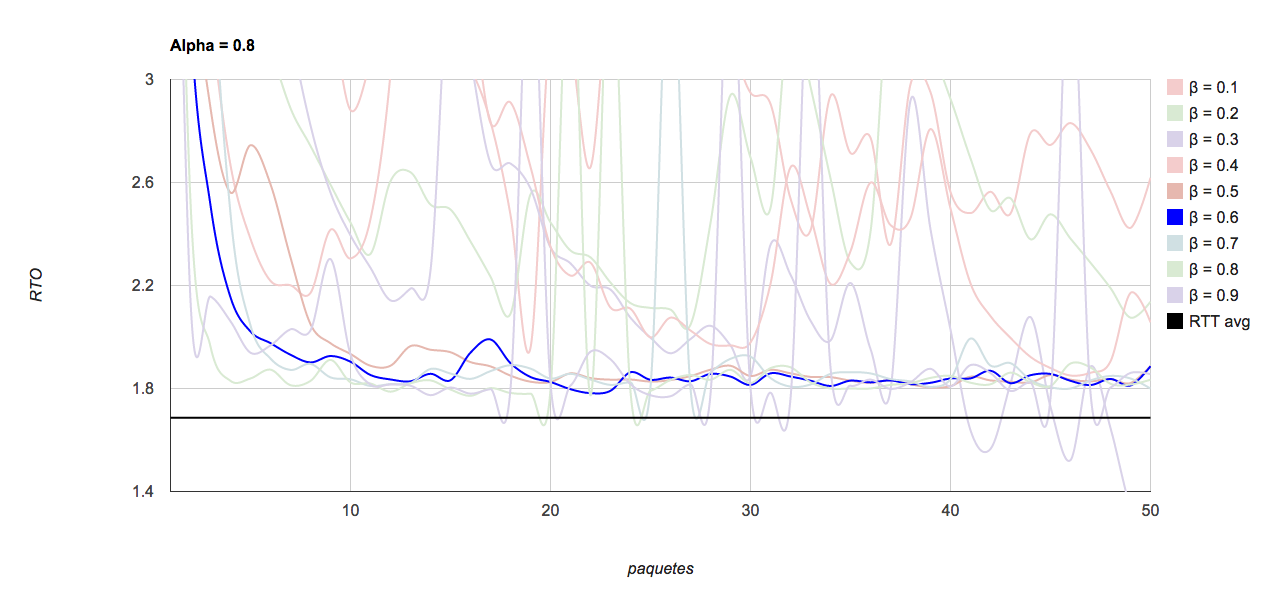
\includegraphics[scale=0.35]{graphics/rto_vs_paquetes_a_8.png}
	\textit{Gráfico interactivo en:} http://goo.gl/RGiQc0
\end{center}

\begin{center}
	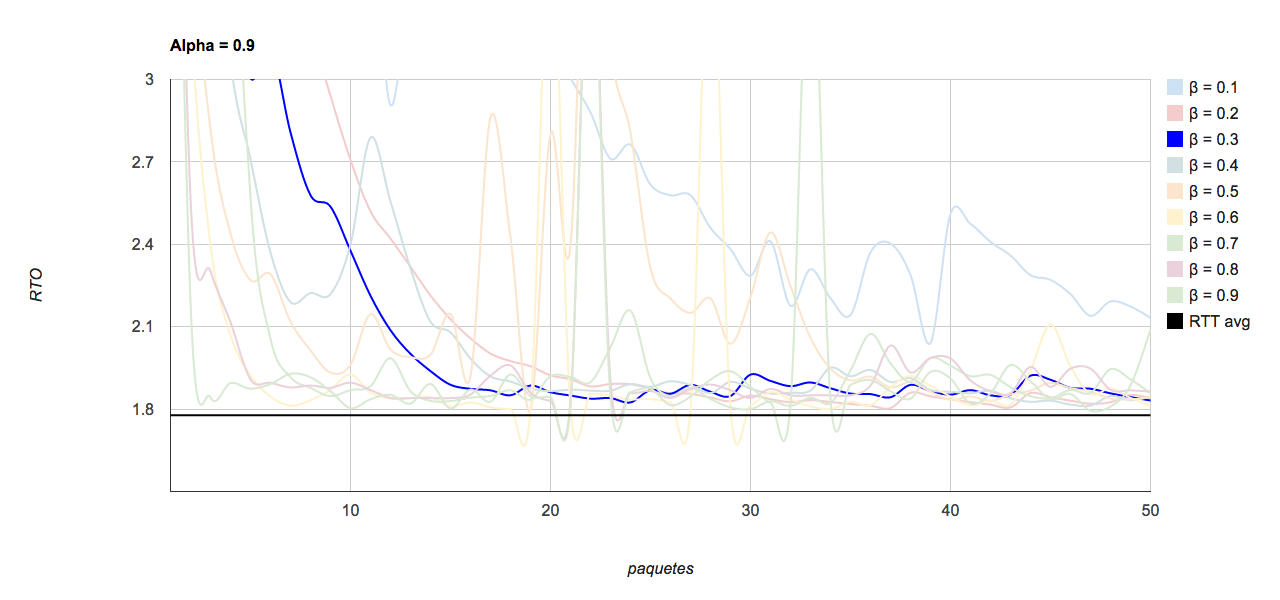
\includegraphics[scale=0.35]{graphics/rto_vs_paquetes_a_9.png}
	\textit{Gráfico interactivo en:} http://goo.gl/QXH7cA
\end{center}

De cada uno de los gráficos, extrajimos el mejor par $\alpha$, $\beta$ y los juntamos en un mismo gráfico para, entre ellos, elegir el mejor de las 81 posibilidades. Según esta experimentación, entonces, los mejores valores en este protocolo para $\alpha$ y $\beta$ en nuestro caso, nos dieron cuando $\alpha = 0.4$ y $\beta = 0.7$.

\begin{center}
	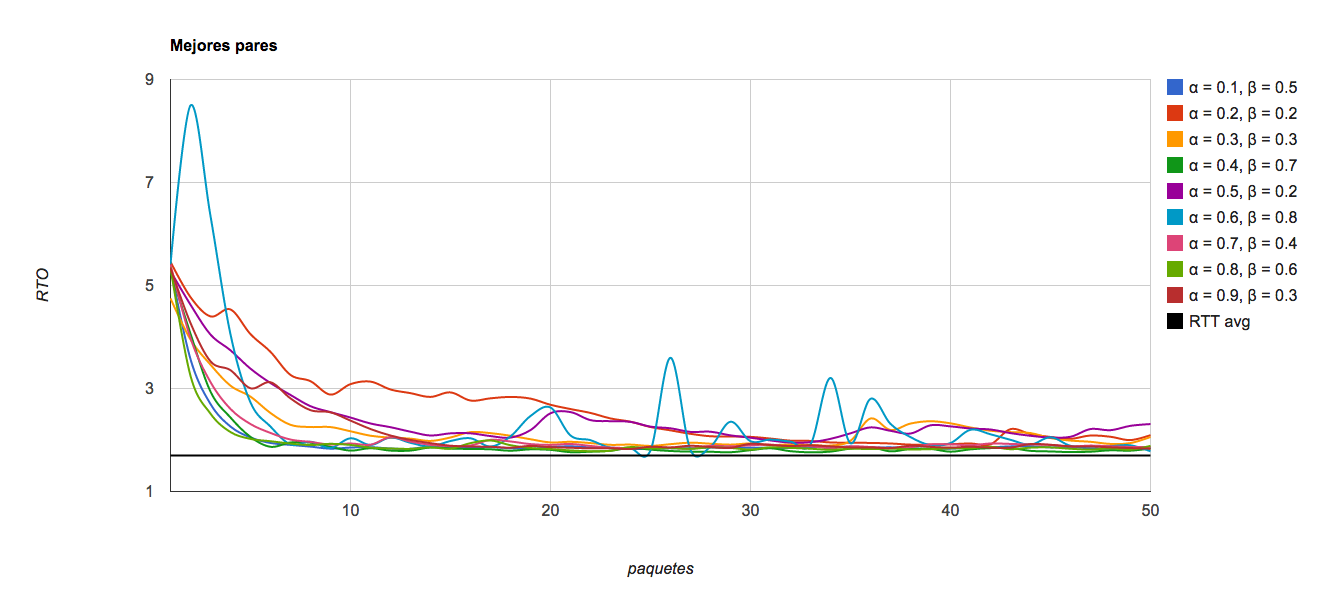
\includegraphics[scale=0.35]{graphics/best_pairs.png}
	\textit{Gráfico interactivo en:} http://goo.gl/FBA1p2
\end{center}

El gráfico anterior lo dejamos para dimensionar la convergencia y los valores en general. El siguiente gráfico es el que realmente hace notar que de todas las opciones, la anteriormente elegida es la que más cerca se encuentra del promedio de RTT, y además, la que más estable mantiene dicha cercanía.

\begin{center}
	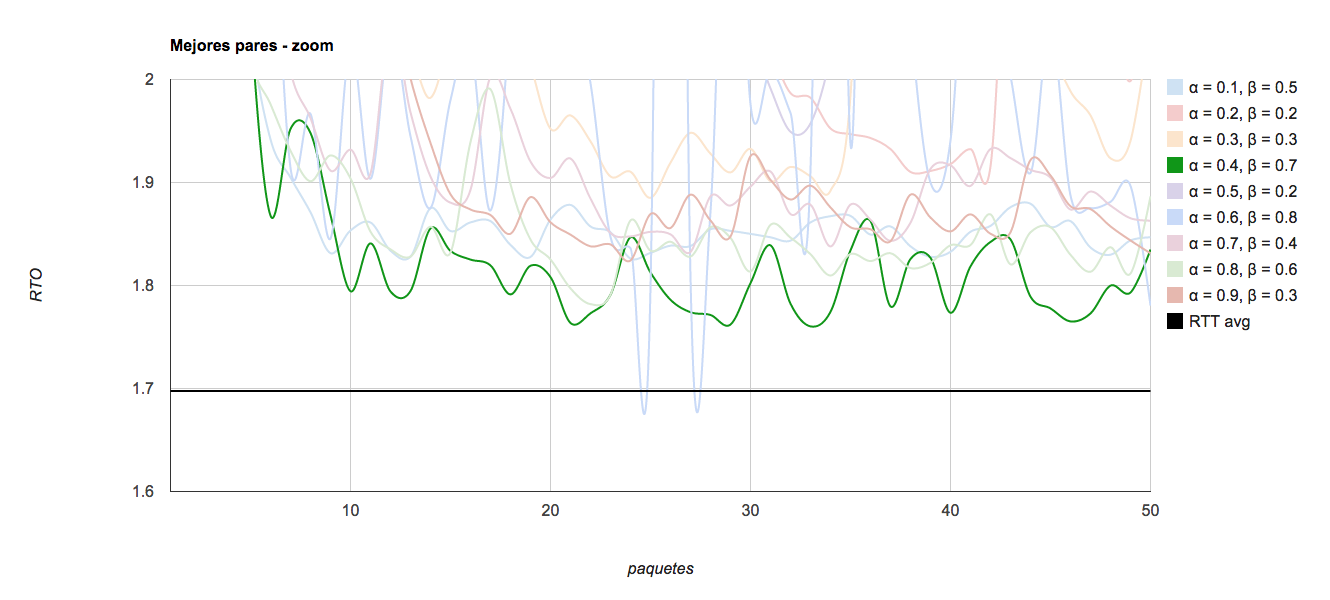
\includegraphics[scale=0.35]{graphics/best_pairs_zoom.png}
	\textit{Gráfico interactivo en:} http://goo.gl/RvuVpr
\end{center}